%----------------------------------------------------------------------------------------
%	Hardware
%----------------------------------------------------------------------------------------

\chapter{Hardware Components}

This section details the hardware design, including research on prior solutions, load cells, sensing and processing circuits, and the proposed design.

\section{Prior Art}

In this section, existing hardware solutions for digital weighing scales are evaluated. 

The 2nd Gen Xiaomi Smart Scale is an intelligent scale that has the primary function of measuring peoples weights, with many extra functions that allow fitness tracking with connected Xiaomi accounts. The technical specifications consist of: High precision pressure sensors that can measure still items over 100g and accurately perceive subtle changes of 50g, Bluetooth 5.0 connectivity for devices to track body information via the Xiaomi sports APP.. This scale’s functionality goes beyond the average scale, with data such as body balance, weight and BMI being uploaded and tracked on the sports app, and diet and fitness plans being issued/adjusted to users. the higher price may not appeal to people that are not willing to spend much on a scale

The Living \& Co Digital Glass Scale is a cheap alternative of a weight scale with little extra functionality. It is for people that only require the bare minimum out of a weight scale, with a “high precision strain-gauge sensor” that will always give you accuracy every time. The functionality of the product is severely limited. This scale is made for people without a bigger budget, or people not willing to invest much in a weight scale. This lack of extra functionality also means that it is easier for people to use, however, it means it is only limited to one function. Bad reviews about massive fluctuations in measurements also sets this product back.

The FItBit Aria Air is a smart scale that functions as a regular weighing scale, but also records weights and synchronises the users biometrics to the FitBit app. The technical specifications consist of: Bluetooth functionality that connects to devices that track body information via the FitBit app. In terms of functionality, the scale syncs the weight to the FitBit app where people can view their trends and see other details recorded by FitBit trackers and watches, such as BMI. FitBit is a very popular health and fitness brand that benefits the user if they have more ways to measure health metrics. Unfortunately, this means that the proprietary applications result in limited competition for already invested FitBit users, and the higher price does not appeal to people that are not willing to spend much on a scale

Generally, all physical weight scales are the same, with differences being in the more expensive range having the ability to connect to other devices where weight metrics are processed with other body measurements to give users more information on their health. This principle can be applied to not only humans, but also dogs. Our focus is to provide the weights of dogs, but also to upload that information to a database where further processing may take place, or purely just to track weight.


\section{Load Cell Working Principles}

A strain gauge is an electrical sensor that reacts to weight by having an electrical resistance that increases or decreases when weight is applied. A load cell uses several strain gauges to measure weight more accurately than one strain gauge. The provided load cells have two strain gauges as in Figure \ref{fig:load_cell}. One’s resistance decreases linearly with weight, and the other’s resistance increases linearly. Four load cells are provided, referred to as R1, R2, R3, and R4.



\begin{figure}[!ht]
	\centering
	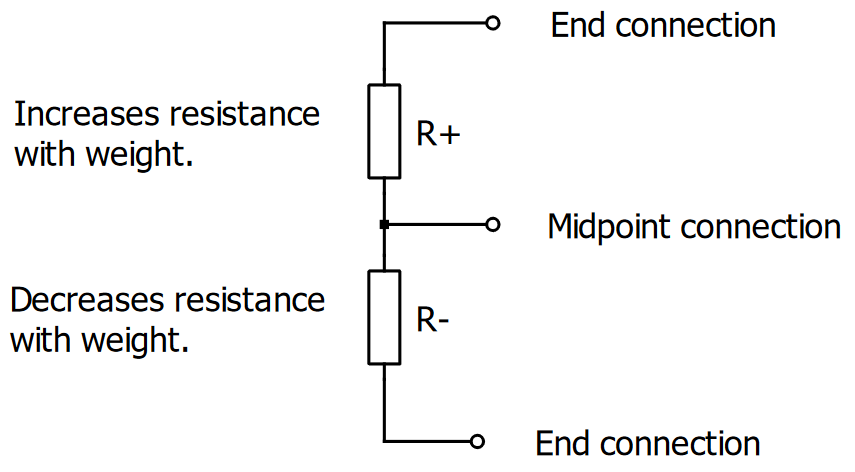
\includegraphics[scale=0.3]{load-cell.png}
	\caption{Diagram of the provided load cell.}
	\label{fig:load_cell}
\end{figure}


\section{Sensing Topologies}

Topologies to connect the load cells are compared. The load cells could individually be connected to the ADC to gain a measurement from each, as in Figure \ref{fig:sense-1}. This would allow weight distribution to be sensed across the scale by gaining measurements from each corner; however, it requires four signals to be input to the ADC. With only three ADC ports, this option is only possible if an external ADC is used at additional cost. Another option is connecting all load cells together in a parallel configuration as in Figure \ref{fig:sense-2} and sending one signal to the ADC. This option is low cost as it only requires one processing circuit. However, parallel connections reduce resolution because each load cell's resistance changes are averaged instead of being added. Alternatively, the load cells could be placed in a Wheatstone bridge as in Figure \ref{fig:sense-3}. This topology is used to detect small changes in resistance and produces a high-resolution output. Adding multiple load cells in the Wheatstone bridge does not reduce resolution because differences are added and not averaged. Further, this option only requires one processing circuit; thus is a low-cost solution. 



\section{Processing Topologies}

Processing the sensed signal required because the signal is small and to meet requirements of the ADC, and of the chosen op-amp. The requirements are: the signal should always be 0 V to 3.3V and an offset to the signal is required for the op-amp output.

To produce an offset, a Zener regulator may be used as in Figure \ref{fig:offset}.a. However, the offset it produces is limited to standard values. Alternatively, resistors may be used to divide the supply voltage down. An op-amp buffer is added to the voltage divider to hold the offset steady as in Figure \ref{fig:offset}.b.

To amplify the signal, an amplifier that allows double ended inputs must be used, as output by the Wheatstone bridge. As such, a differential amplifier as in Figure \ref{fig:amplifier} would be suitable. However, its output can vary depending on the load cells' resistances so to prevent this, an instrumentation amplifier is used as in Figure \ref{fig:amplifier-2}.


\section{The Proposed Design}

The proposed design comprises a Wheatstone bridge and instrumentation amplifier as in Figure \ref{fig:schematic}. The design was simulated with results in Figure \ref{fig:simulation}. Values from practical testing were used for the load cell characteristics. The output varies linearly, and is amplified and offset successfully. Functional specifications include a 3.3 V operating voltage, 0 to 25 kg range, and 0.5 kg resolution. Technical specifications include a 714 V/V gain, 0.1 V offset, and 0.8 V to 1.8 V range.


\begin{figure}[!ht]
	\centering
	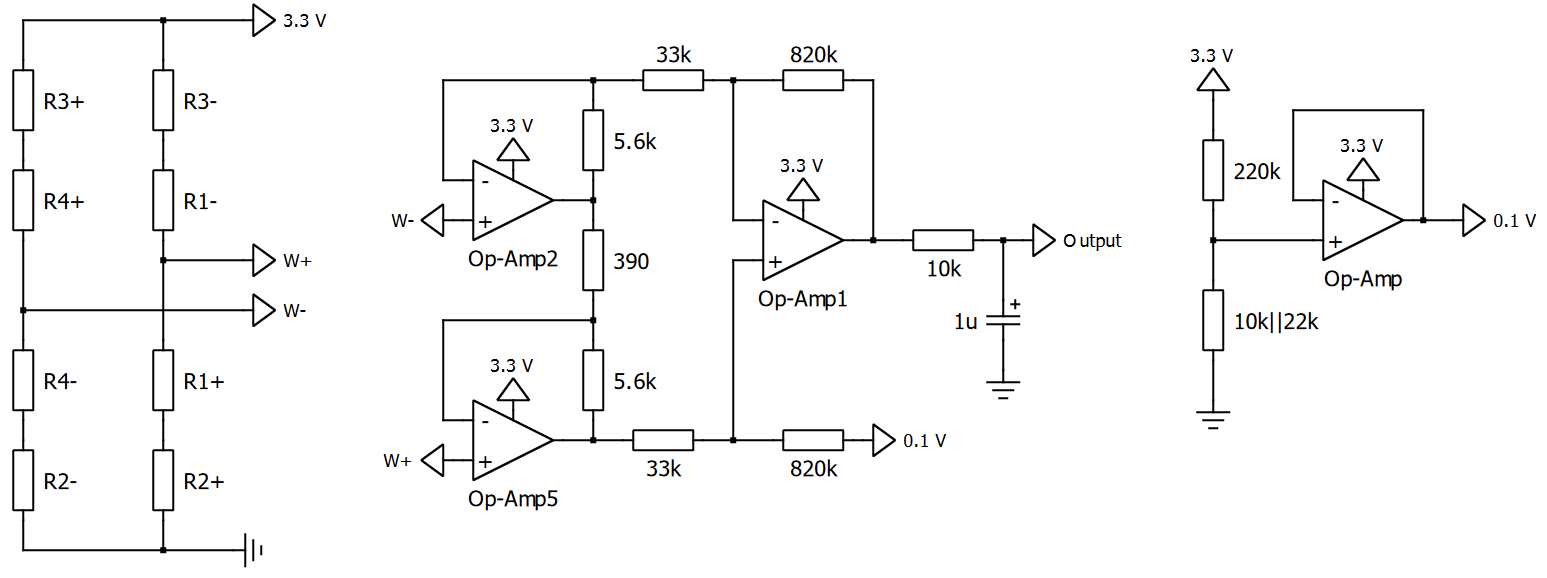
\includegraphics[scale=0.33]{schematic.png}
	\caption{Hardware schematic.}
	\label{fig:schematic}
\end{figure}

\begin{figure}[!ht]
	\centering
	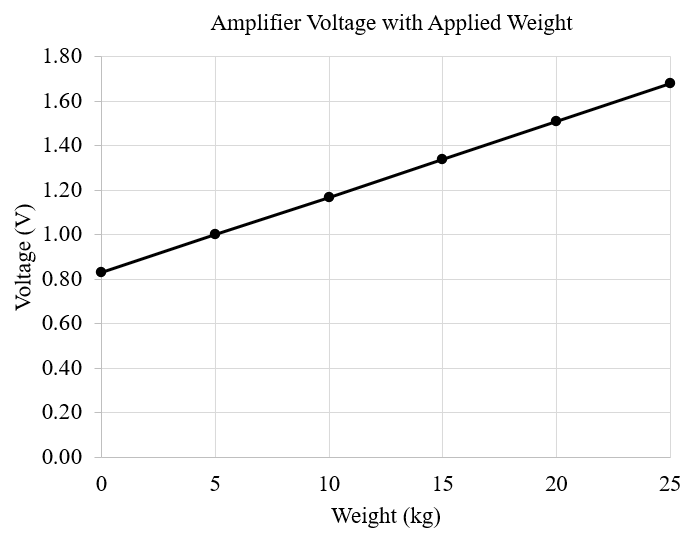
\includegraphics[scale=0.37]{simulation.png}
	\caption{Hardware simulation results.}
	\label{fig:simulation}
\end{figure}



